\newpage
\section{Bijlage}

\subsection*{User Story}
Nadat de robot de ruimte in kaart heeft gebracht en de optimale route bepaald
heeft, moet dit allemaal op een manier toegankelijk worden gesteld aan de
gebruiker.

Dit zal gedaan worden d.m.v. het hosten van een web interface op een aparte
“server PI”. Deze PI zal vervolgens ook een manier van communicatie opstellen
met de roomba PI om vervolgens hun informatie met elkaar te delen.

\subsection*{UML modellen}
\label{ssec:uml model voor de api server}
\begin{figure}[H]
    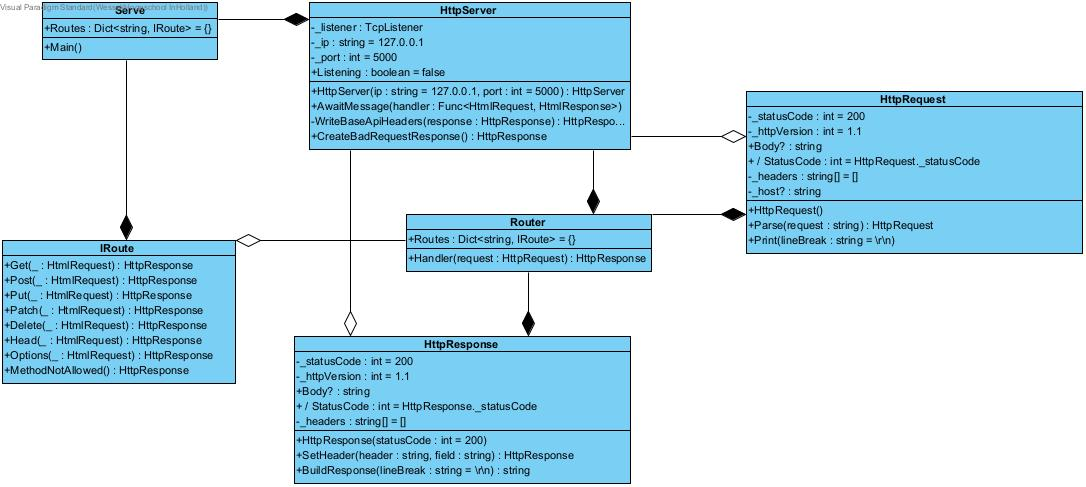
\includegraphics[width=1\textwidth]{uml-v1.jpg}
    \caption{1\textsuperscript{e} versie UML model.}
    \label{fig:umlv1}
\end{figure}

\newpage

\begin{figure}[H]
    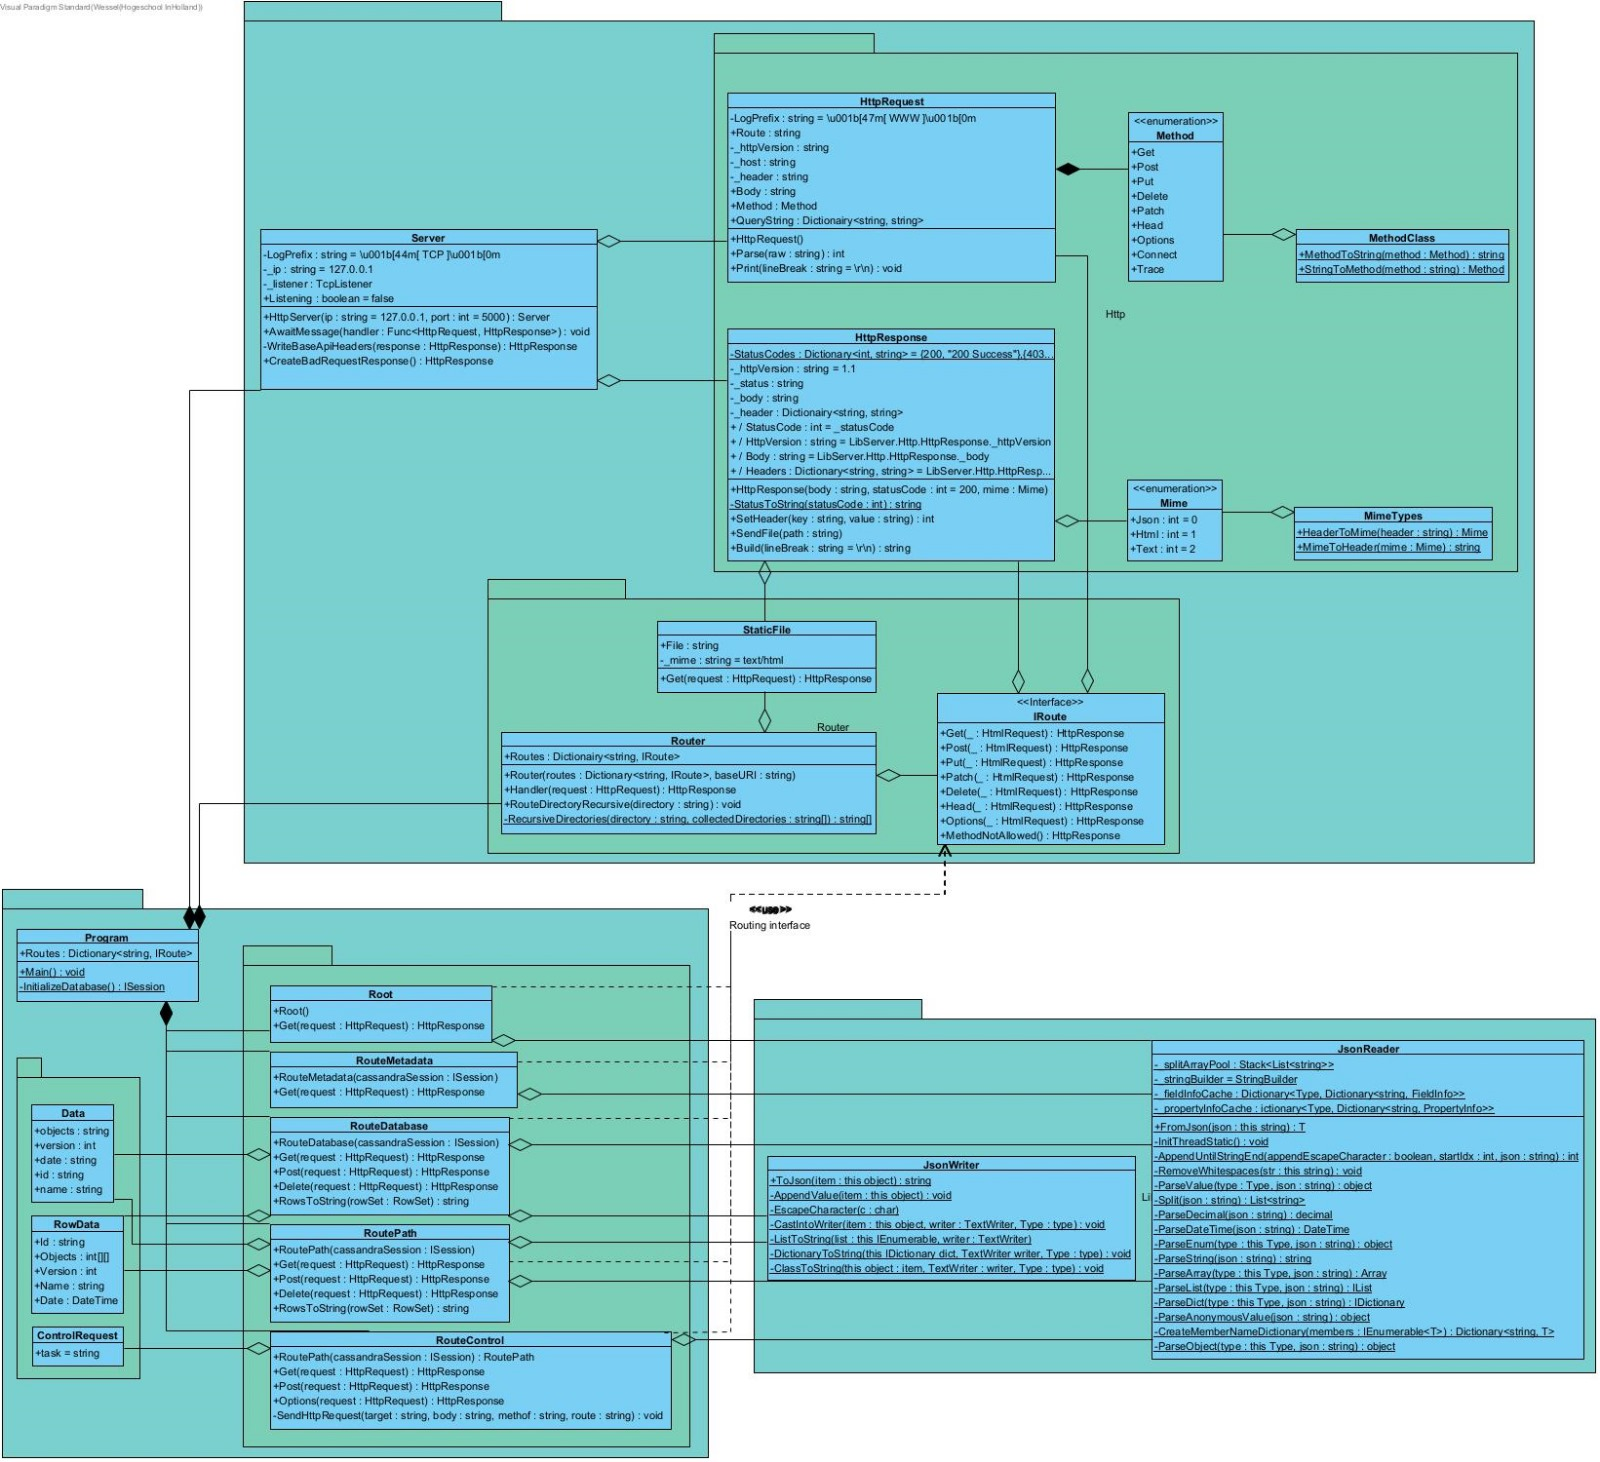
\includegraphics[width=1\textwidth]{uml.jpg}
    \caption{Uiteindelijke versie UML model.}
    \label{fig:uml}
\end{figure}

\newpage
